\documentclass[output=paper]{langsci/langscibook}
\ChapterDOI{10.5281/zenodo.3972842}

\author{Eric Haeberli\affiliation{University of Geneva}\lastand Tabea Ihsane\affiliation{University of Geneva}}
\title{Micro- and nano-change in the verbal syntax of English}

% \chapterDOI{} %will be filled in at production

\abstract{The verbal syntax of \ili{English} undergoes substantial changes in the
    Late Middle and \ili{Early Modern English} periods. The outcome of these changes
    is a clear division between main verbs and auxiliaries with respect to
    their syntactic behaviour. On the basis of quantitative data tracing the
    diachronic development of the distribution of verbal elements with respect
    to \isi{adverbs}, this paper argues that the path towards the present-day system
    with a separate syntactic class of auxiliaries involved several small-scale
steps that can be considered to be of the micro-\is{parameters} and nano-type in
\citeauthor{BibRob2012b}'s (\citeyear{BibRob2012b,BibRob2016}) terminology.}

\maketitle

\begin{document}\glsresetall

%\textbf{Keywords:}

\section{Introduction}\largerpage

As is well known, the verbal syntax of \ili{English} undergoes important changes in
the transition from Middle to \ili{Early Modern English}. On the one hand, finite
main verbs stop moving to the inflectional domain (decline of V-movement\is{verb movement}, cf.\
\citealt{Roberts1985,Roberts1993,Kroch1989,Pollock1989} among many others),
and, on the other hand, auxiliaries start forming a clearly distinct class of
elements (recategorization of auxiliaries, cf.\ e.g.\
\citealt{Lightfoot1979,Lightfoot2006b,Warner1993}). In this paper, we will
examine how these two developments interact, and we will show that what has
generally been treated as major syntactic changes may have involved smaller
steps with brief periods of variation at what, in \citeauthor{BibRob2012b}'s
(\citeyear{BibRob2012b,BibRob2016}) terms, could be called the
micro-\is{parameters} and nano-parametric level.

Our evidence comes from the distribution of finite verbal elements and \isi{adverbs}.
Besides negation, \isi{adverbs} have been considered as the main diagnostic for
V-movement out of the VP to the inflectional domain, the assumption being that
certain \isi{adverbs} and negation are merged above the VP and that the occurrence of
the verb to the left of these is a sign of V-movement\is{verb movement} whereas the occurrence of
the verb to the right signals the absence of such movement (cf.\
\citealt{Emonds1978,Pollock1989} among many others). In the literature on the
loss of V-movement\is{verb movement} in the history of \ili{English}, discussions have generally
focussed mainly on negation and the rise of \emph{do}-support.  In
\citet{HaeIhs2016}, data involving \isi{adverbs} are examined in detail, and
it is shown that the two diagnostics for V-movement\is{verb movement} do not pattern alike.
Whereas V-movement\is{verb movement} past \isi{adverbs} declines relatively quickly between the middle
of the 15th century and the middle of the 16th century, the loss of V-movement
past negation starts only in the 16th century and takes well into the 18th
century to be completed. On the basis of this contrast, Haeberli \& Ihsane
conclude that the loss of V-movement\is{verb movement} in the history of \ili{English} is a two-step
process (cf.\ also \citealt{Han2000,HanKro2000} for this claim based on
different evidence). In the first phase, around 1500, V-movement\is{verb movement} to a high
inflectional head is lost (T in Haeberli \& Ihsane’s analysis) whereas
V-movement to a low inflectional head is maintained (Asp). This leads to a
situation where V-movement\is{verb movement} past \isi{adverbs} is lost while movement past negation
still remains productive. Then, in the second phase, V-movement\is{verb movement} out of the VP
is lost entirely and finite main verbs no longer occur to the left of negation.

Given that the first phase in the loss of V-movement\is{verb movement} starts in the 15th
century, we would expect it to interact with the second major change affecting
the verbal syntax in \ili{Early Modern English}, i.e.\ the change in the syntactic
status of auxiliaries. It is generally assumed in the literature that
auxiliaries belong to the category V in early \ili{English}, but that they are then
reanalysed as belonging to a functional category in \ili{Early Modern English}. For
modals, this change has been situated approximately in the early 16th century
\parencites[cf.\
e.g.][110]{Lightfoot1979}[31]{Lightfoot2006b}[310f.]{Roberts1993}. Since the
decline of V-movement\is{verb movement} past \isi{adverbs} already starts in the 15th century, we would
expect that auxiliaries first participate in this change, but that they stop
doing so with the categorial \isi{reanalysis} in the early 16th century. In the
following section, we will examine the diachronic development of adverb
placement with respect to auxiliaries in order to determine whether such an
interaction between the decline of V-movement\is{verb movement} and the recategorization of
auxiliaries can indeed be observed.\footnote{An anonymous reviewer suggests
    that the interaction between the loss of \isi{verb movement} and the
    recategorization of auxiliaries should also be tested on the basis of
    subject--verb inversion contexts as found in questions, where the verb must
    move out of the VP to reach a higher V2 position in the CP-domain. However,
    it is not clear whether subject--verb inversion data would provide us with
    useful evidence for the purposes of our investigation. First, the Mainland
    Scandinavian languages suggest that finite verbs can still move to C even
    after the loss of V-to-T\is{verb movement} movement. And secondly, although standard
    generative accounts assume that a verb has to move through the inflectional
    domain on its way to C, direct movement to C would be conceivable in more
    recent frameworks (cf.\ e.g.\ \citealt{Roberts2012b} for an approach that
    allows movement from one phase head to another (i.e.\ v-to-C); or cf.\ also
    approaches viewing V2 as a \gls{PF} phenomenon). Given these observations, it
    seems that the adverb data considered below provide more solid evidence for
    our purposes than subject--verb inversion data. However, it would no doubt
    be worth exploring the consequences of the findings in
    \citet{HaeIhs2016} and in this paper with respect to how V-movement
to C developed in the history of \ili{English}, but we will have to leave this issue
for future research.}

\section{Adverb placement with different types of verbal elements}

Old and Early \ili{Middle English} had relatively frequent occurrences of adverbs
between a subject and a finite main verb (SAdvV order) due to a certain
variability in subject and verb placement. This system is simplified in the
course of the \ili{Middle English} period, and the subject and the finite verb are
increasingly adjacent. In structural terms and under the assumption that
adverbs are diagnostics for V-movement\is{verb movement}, this development can be considered as a
trend towards a French-style grammar in which the verb moves past \isi{adverbs} to T
and the subject occurs in Spec,TP in non-interrogative clauses (cf.\
\citealt[531ff.]{HaeIhs2016} for discussion). In the middle of the 15th
century, however, this trend is inverted and the frequency of the word order
SAdvV increases again. In the data presented by \citet[512]{HaeIhs2016}, the
rate of SAdvV measured against the total number of clauses with an adverb to
the right of the subject reaches its lowest point in the period 1420--1475
(8.5\%). This rate increases to 16.5\% in the period 1475--1500 and to 37.3\% in
the period 1500--1525, both changes being statistically significant. This quick
rise of medial adverb placement, which is followed by a certain stability, can
be considered as a symptom of the loss of V-movement\is{verb movement} past \isi{adverbs}. The fact
that SVAdv is not entirely lost is due to an alternative option to derive this
word order that is independent of V-movement\is{verb movement} and that remains in use until
today (right-\isi{adjunction} of the adverb in the traditional account). There are
contexts, however, in which a word order option depends entirely on the
presence of V-movement\is{verb movement}, and these contexts provide support for the hypothesis
that V-movement\is{verb movement} past \isi{adverbs} is lost around 1500 (cf.\
\citealt[514--520]{HaeIhs2016}). Adverb placement with finite main verbs can
then be taken as a baseline against which to examine the development of
auxiliaries.\footnote{In this paper and in \citet{HaeIhs2016}, we include data
    involving any type of adverb in our counts. A reviewer considers this as
    potentially problematic as different types of \isi{adverbs} might occur in
    different positions in the clause structure. Two observations can be made
    here.  First, given that one of the crucial word orders examined below
    (SAdvAuxV) occurs with very low frequencies, a further subdivision of the
    data according to adverb types would not allow us to obtain any meaningful
    results, possibly even if we extended our corpus substantially. However,
    even if the amount of available data were larger, it is not clear whether
    adverb type indeed interferes in a significant way with the change
    considered here. Data involving finite verbs and \isi{adverbs} are more abundant,
and with those no clear adverb type effect can be detected (cf.
\citealt[516--520, 524--525]{HaeIhs2016} for discussion).} Assuming that
auxiliaries have the same categorial status as main verbs in early \ili{English}, we
expect their distribution with respect to \isi{adverbs} to develop in parallel until
the two types of elements become categorially distinct.

\subsection{Modals}

\textcite{HaeIhsta} examine the development of the distribution of
modals with respect to \isi{adverbs}. One of their findings is that, throughout Old
and \ili{Middle English}, the frequency of the order SAdvM(odal)V measured against
SMAdvV and SMVAdv is considerably lower than the frequency of SAdvV measured
against SVAdv. Although this quantitative difference could be interpreted as
suggesting that modals do not occur in the same structural position and thus do
not have the same categorial status as main verbs already in early \ili{English},
Haeberli \& Ihsane show that such a conclusion is not necessarily correct and
that other factors may play an important role in the quantitative contrast. If
this is the case, the comparison should rather focus on the general diachronic
trajectories, and in this respect the two contexts turn out to match up to
1500. This is shown in \Cref{tab:key:09.1}, which presents data for adverb
placement with respect to finite modals from 1350 to 1650 (from Haeberli \&
Ihsane to appear) and compares them with main verbs
(frequencies in the final column from \citealt[512]{HaeIhs2016}).\footnote{The
    data in the tables in this paper are based on the following three parsed
    corpora: \emph{The Penn--Helsinki Parsed Corpus of Middle \ili{English} 2}
    (\gls{PPCME2} (1150--1500); \citealt{KroTay2000}), \emph{The Parsed Corpus
    of Early \ili{English} Correspondence} (\gls{PCEEC} (c.\ 1410--1695);
    \citealt{TaylorEtAl2006}), and \emph{The Penn--Helsinki Parsed Corpus of
    Early Modern English} (\gls{PPCEME} (1500--1700); \citealt{KrochEtAl2010}).
    Overlaps between PCEEC and PPCEME have been removed.  The data cover all
    main and subordinate clauses with an overt subject and a one-word AdvP of
    any type.  In addition to the elements referred to in the word order
    patterns (S, A(dv), V, M(odal), \emph{be}, \emph{have}), further
    constituents such as objects, adjuncts or, in clauses with an
    auxiliary\is{auxiliaries}, a second non-finite element may occur in any position in
    these clauses. An anonymous reviewer points out that it might be
    problematic to collapse main clause and subordinate clause data as the two
    clause types may behave differently with respect to adverb placement. For
    the auxiliary\is{auxiliaries} data, this concern does not seem to be warranted. If we
    take all main and subordinate clauses containing an adverb and a finite
    auxiliary\is{auxiliaries} (excluding copula\is{copulas} \emph{be}) and we measure the rate of
    SAdvAuxV order in the two clause types separately, we can observe that
    between 1350 and 1650 the frequency of SAdvAuxV order indeed tends to be
    slightly higher in subordinate clauses but that this contrast is
    statistically significant in only one of the subperiods (1525--1550). To
    collapse main and subordinate clauses does therefore not seem to alter the
    general diachronic picture we obtain and it has the advantage of increasing
    the sample sizes. As for the baseline with finite main verbs, the clause
    type difference is somewhat more important (cf.\ \citealt[524, fn.\
    52]{HaeIhs2016}) in that SAdvV order is significantly more frequent in
    subordinate clauses in 5 of the 9 subperiods between 1350 and 1650.
    However, the general diachronic trajectory is similar, with SAdvV order
    sharply rising in the periods 1475--1500 and 1500--1525 in both clause types
    and with the frequencies then remaining, with some fluctuations, at the
    same level.  For our purposes, it is this general diachronic picture that
    is essential.  Distinguishing clause types would not alter our conclusions
in any substantial way.}

\begin{table}
\caption{The distribution of finite modals and \isi{adverbs} following an overt
    subject in Late Middle and \ili{Early Modern English} (PPCME2, PCEEC,
PPCEME)\label{tab:key:09.1}}
\begin{tabular}{lrrrrrr}
\lsptoprule
{Period} & {SAMV} & {SMAV} & {SMVA} & {Total} & {\%SAMV} & {\%SAV}\\
\midrule
1350--1420 & 26 & 312 & 266 & 604 & 4.3 & 9.9\\
1420--1475 & 10 & 419 & 484 & 913 & 1.1 & 8.5\\
1475--1500 & 14 & 159 & 185 & 358 & 3.9 & 16.5\\
1500--1525 & 4 & 177 & 114 & 295 & 1.4 & 37.3\\
1525--1550 & 19 & 553 & 375 & 947 & 2.0 & 33.9\\
1550--1575 & 28 & 453 & 316 & 797 & 3.5 & 34.9\\
1575--1600 & 20 & 661 & 386 & 1067 & 1.9 & 34.0\\
1600--1625 & 18 & 706 & 386 & 1110 & 1.6 & 40.9\\
1625--1650 & 21 & 686 & 475 & 1182 & 1.8 & 39.8\\
\lspbottomrule
\end{tabular}
\end{table}

The periods 1350--1420 and 1420--1475 show the end of a gradual decline in the
frequencies of SAdvMV and SAdvV order from \ili{Old English} onwards, with the low
point being reached in 1420--1475.\footnote{For the \ili{Old English} and Early
Middle \ili{English} data, cf.\ \textcites[512]{HaeIhs2016}{HaeIhsta}.}  In the
following period 1475--1500, we see a significant increase of SAdvX both with
modals ($\chi^2$: 11.00, $p < 0.001$) and with main verbs ($\chi^2$: 36.35, $p
< 0.001$). But whereas this rise continues with main verbs in the period
1500--1525 and the frequencies then remain relatively stable, the rate of SAdvMV
order drops in a statistically significant way to the level before 1475
($\chi^2$: 3.94, $p < 0.05$). After that, there are two small increases with
SAdvMV order but neither of them reaches statistical
significance.\footnote{Comparisons of the different periods give the following
    results: 1500--1525 vs.\ 1525--1550: $\chi^2$ = 0.52; $p < 0.5$; 1525--1550 vs.
    1550--1575: $\chi^2$ = 3.75, $p = 0.053$; 1500--1525 vs.\  1550--1575:
$\chi^2$ = 3.52, $p = 0.061$.} Finally, SAdvMV stabilizes at a slightly lower
level.

From a structural point of view, the developments in \Cref{tab:key:09.1} can be
interpreted as follows. As shown by \citet{HaeIhs2016}, the increase in SAdvV
order with main verbs around 1500 is best analysed as a symptom of the loss of
V-movement. The same could then be said for the parallel development with
modals in the period 1475--1500. At this point, modals still have the status of
verbs and V-movement\is{verb movement} past \isi{adverbs} therefore declines, leading to an increase in
{SAdvMV} order. In the following period, however, modals start being reanalysed
as elements merged (presumably relatively high) in the functional domain and
the order SAdvMV therefore declines again. This analysis thus identifies
exactly the same moment in time for the recategorization of the modals (i.e.\
the early 16th century) as earlier proposals made in the literature on the
basis of entirely independent evidence \parencites[cf.\
e.g.][110]{Lightfoot1979}[31]{Lightfoot2006b}[310f.]{Roberts1993}.
%
%(cf.\ e.g.\ \citealt{Lightfoot1979}: 110, 2006: 31, \citealt{Roberts1993}:
%310f.).

\subsection{\emph{be}}

Let us now consider the behaviour of other auxiliaries with respect to adverb
placement. In early \ili{English}, auxiliary\is{auxiliaries} \emph{be} can co-occur with a main
verb in the present participle form or the past participle form, and with the
latter both in the active and the passive voice. Our corpus contains too few
examples with present participles and the active voice to allow for meaningful
separate quantitative analyses. \Cref{tab:key:09.2} therefore combines the three
contexts and thus covers clauses with finite \emph{be} and any non-finite
main verb.

\begin{table}
\caption{The distribution of auxiliary\is{auxiliaries} \emph{be} and \isi{adverbs} following an
overt subject in Late Middle and \ili{Early Modern English} (PPCME2, PCEEC, PPCEME)}%
\label{tab:key:09.2}
\begin{tabular}{lrrrrr}
\lsptoprule
{Period} & {SA\emph{be}V} & {S\emph{be}AV} & {S\emph{be}VA} & {Total} & {\%SA\emph{be}V}\\
\midrule
1350--1420 & 19 & 232 & 161 & 412 & 4.6\\
1420--1475 & 8 & 327 & 147 & 482 & 1.7\\
1475--1500 & 2 & 157 & 65 & 224 & 0.9\\
1500--1525 & 8 & 150 & 56 & 214 & 3.7\\
1525--1550 & 5 & 264 & 123 & 392 & 1.3\\
1550--1575 & 10 & 291 & 109 & 410 & 2.4\\
1575--1600 & 11 & 374 & 117 & 502 & 2.2\\
1600--1625 & 8 & 398 & 117 & 523 & 1.5\\
1625--1650 & 8 & 329 & 103 & 440 & 1.8\\
\lspbottomrule
\end{tabular}
\end{table}

As with modals, we see an initial decline in SAdv\emph{be}V order. However,
in contrast to the modals, the low point of 0.9\% is reached only in the period
1475--1500 rather than in the period 1420--1475. But subsequently we see the same
quantitative pattern as with modals: a rise to 3.7\% followed by an immediate
decline to 1.3\%.\footnote{These two developments do not quite reach
statistical significance, however (rise in 1500--1525: two-tailed Fisher exact
test, $p = 0.057$; decline in 1525--1550: two-tailed Fisher exact test, $p =
0.073$).}\largerpage

The development of auxiliary\is{auxiliaries} \emph{be} can now be compared to that of copula\is{copulas}
\emph{be}. \Cref{tab:key:09.3} presents data involving copula\is{copulas} \emph{be}
followed by some non-verbal {predicate}.{\interfootnotelinepenalty=10000\footnote{Clauses with an elided
    predicate are not included. Furthermore, we also excluded clauses of the
type \emph{It so is that …} as some early texts use them repeatedly without
variation in adverbial placement and the regular occurrences of these clauses
would distort the general picture somewhat.}}\newpage

\begin{table}
\caption{The distribution of copula\is{copulas} \emph{be} and \isi{adverbs} following an overt
subject in Late Middle and \ili{Early Modern English} (PPCME2, PCEEC,
PPCEME)\label{tab:key:09.3}}
\begin{tabular}{lrrrr}
\lsptoprule
{Period} & {SA\emph{be}} & {S\emph{be}A} & {Total} & {\%SA\emph{be}}\\
\midrule
1350--1420 & 17 & 189 & 206 & 8.3\\
1420--1475 & 4 & 270 & 274 & 1.5\\
1475--1500 & 2 & 139 & 141 & 1.4\\
1500--1525 & 8 & 77 & 85 & 9.4\\
1525--1550 & 17 & 220 & 237 & 7.2\\
1550--1575 & 13 & 224 & 237 & 5.5\\
1575--1600 & 11 & 218 & 229 & 4.8\\
1600--1625 & 15 & 331 & 346 & 4.3\\
1625--1650 & 21 & 393 & 414 & 5.1\\
\lspbottomrule
\end{tabular}
\end{table}

Once again, we see an initial decline which, as in the case of auxiliary\is{auxiliaries}
\emph{be}, reaches its low point in the period 1475--1500 with 1.4\%
SAdv\emph{be} order. Then, there is a statistically significant rise to 9.4\%
(two-tailed Fisher exact test, $p = 0.007$) and a subsequent decline that is
gradual over several periods.

\subsection{\emph{have}}

Finally, consider adverb placement in clauses with the finite auxiliary\is{auxiliaries}
\emph{have} and a main verb in the past participle form. The relevant
quantitative data are provided in \Cref{tab:key:09.4}.

\begin{table}
\caption{The distribution of auxiliary\is{auxiliaries} \emph{have} and \isi{adverbs} following an
overt subject in Late Middle and \ili{Early Modern English} (PPCME2, PCEEC,
PPCEME)\label{tab:key:09.4}}
\begin{tabular}{lrrrrr}
\lsptoprule
{Period} & {SA\emph{have}V} & {S\emph{have}AV} & {S\emph{have}VA} & {Total} & {\%SA\emph{have}V}\\
\midrule
1350--1420 & 2 & 69 & 109 & 180 & 1.1\\
1420--1475 & 5 & 85 & 174 & 264 & 1.9\\
1475--1500 & 2 & 49 & 66 & 117 & 1.7\\
1500--1525 & 6 & 65 & 42 & 113 & 5.3\\
1525--1550 & 26 & 191 & 135 & 352 & 7.4\\
1550--1575 & 17 & 199 & 148 & 364 & 4.7\\
1575--1600 & 11 & 261 & 158 & 430 & 2.6\\
1600--1625 & 11 & 257 & 145 & 413 & 2.7\\
1625--1650 & 7 & 272 & 148 & 427 & 1.6\\
\lspbottomrule
\end{tabular}
\end{table}

The rate of SAdv\emph{have}V is already very low in the initial period
1350--1420. It then remains low up to 1500 and rises in two steps to 5.3\% and
7.4\%. Whereas the first increase is not statistically significant, the
difference between 1475--1500 and 1525--1550 is ($\chi^2$: 5.04, $p = 0.024$).
After 1550, the rate of SAdv\emph{have}V declines. The change is not
statistically significant if we compare adjacent periods but the contrast
between the periods 1525--1550 and 1575--1600 is clearly significant
($\chi^2$: 10.01, $p = 0.002$).

As with \emph{be}, we may now compare the auxiliary\is{auxiliaries} data with those for the
main verb uses. \Cref{tab:key:09.5} shows the distribution of main verb
\emph{have} with respect to \isi{adverbs}.

\begin{table}
\caption{The distribution of main verb \emph{have} and \isi{adverbs} following an
overt subject in Late Middle and \ili{Early Modern English} (PPCME2, PCEEC, PPCEME)\label{tab:key:09.5}}
\begin{tabular}{lrrrr}
\lsptoprule
{Period} & {SA\emph{have}} & {S\emph{have}A} & {Total} & {\%SA\emph{have}}\\
\midrule
1350--1420 & 7 & 57 & 64 & 10.9\\
1420--1475 & 8 & 109 & 117 & 6.8\\
1475--1500 & 1 & 39 & 40 & 2.5\\
1500--1525 & 5 & 34 & 39 & 12.8\\
1525--1550 & 15 & 62 & 77 & 19.5\\
1550--1575 & 12 & 42 & 54 & 22.2\\
1575--1600 & 16 & 68 & 84 & 19.0\\
1600--1625 & 18 & 72 & 90 & 20.0\\
1625--1650 & 21 & 64 & 85 & 24.7\\
\lspbottomrule
\end{tabular}
\end{table}

The frequency of SAdv\emph{have} order declines until the end of the 15th
century. It then rises in the following three periods and remains stable around
20\% until 1650. Thus, up to 1550, auxiliary\is{auxiliaries} \emph{have} and main verb
\emph{have} undergo similar developments.

\subsection{Discussion}\largerpage

\Cref{fig:key:09.1} summarizes the findings reported in Tables 1 to 5. The dates
for the different data points correspond to the middle of each period
distinguished in the tables (e.g.\ 1448 for the period 1420--1475).

\begin{figure}
\caption{Frequency of pre-verbal/pre-auxiliary/pre-copula placement
of \isi{adverbs} in Late Middle and Early Modern English\label{fig:key:09.1}}
\pgfplotstableread{data/HaeberliIhsane.csv}{\table}
\pgfplotstablegetcolsof{\table}
\pgfmathtruncatemacro\numberofcols{\pgfplotsretval-1}
% %     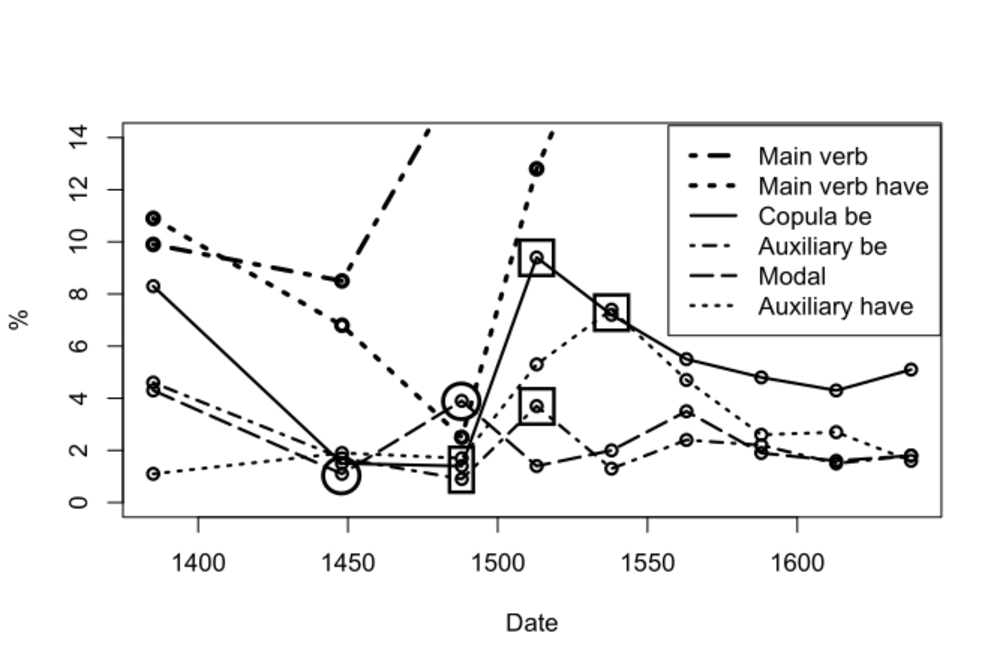
\includegraphics[width=\textwidth]{./img/09-fig1-2.pdf}
\begin{tikzpicture}
  \begin{axis}[
        colormap/RdYlBu,
        cycle list name = langsci,
        height = .45\textheight,
        legend cell align=left,
        legend columns=3,
        legend style={font=\footnotesize,anchor=north,at={(0.5,1.2)},anchor=north},
        line width=.75pt,
        sharp plot,
        width  = \textwidth,
        xlabel = {Date},
        x tick label style={/pgf/number format/1000 sep=},
        xmin = 1380,
        xmax = 1650,
        xtick = {1400,1450,1500,1550,1600},
        ylabel={\%},
        ymin=0,
        ymax=25,
    ]
    \foreach \i in {1,...,\numberofcols} {
                \addplot+ table [x index={1},y index={\i},x expr=\thisrow{Date}] {\table};
                \pgfplotstablegetcolumnnamebyindex{\i}\of{\table}\to{\colname} % Adding column headers to legend
                \addlegendentryexpanded{\colname}
            }
  \end{axis}
\end{tikzpicture}
\end{figure}

            

One might wonder whether these low-frequency data, where potentially relevant
differences occasionally lack statistical significance, allow us to draw any
reliable conclusions. Although it is impossible to fully dispel such concerns
without substantially extending our database, it is nevertheless extremely
striking how regular the quantitative patterns in \Cref{fig:key:09.1} are. With
each type of auxiliary\is{auxiliaries} and copula\is{copulas} \emph{be}, we can first detect a phase of
decline in adverb placement to the left, then a very brief rise of this word
order, and finally another decline. This pattern seems to be too regular to be
entirely accidental.

Interestingly, this common pattern does not occur entirely in parallel across
the different contexts. SAdvMV order (circled data points in
\Cref{fig:key:09.1}) rises together with SAdvV in the period 1475--1500. It
immediately declines again in the period 1500--1525 while SAdvV keeps rising. As
for \emph{have} and \emph{be} (rectangle and squares in
\Cref{fig:key:09.1}), their frequencies for adverb placement to the left remain
low in the period 1475--1500 (rectangle in \Cref{fig:key:09.1}). The rise occurs
in the period 1500--1525 and is thus delayed by one period compared to modals
and main verbs. Finally, the decline of SAdv\emph{be}(V) order is also
delayed by one period compared to modal verbs (1525--1550 rather than 1500--1525)
and the decline with SAdv\emph{have}V starts even later (squares
corresponding to peaks in \Cref{fig:key:09.1}). Thus, we have the sequence main
verb/modals > \emph{have}/\emph{be} for the rise of SAdvX order and the
sequence modal > \emph{be} > auxiliary\is{auxiliaries} \emph{have} for the decline of
SAdvX.\largerpage[-1]

These observations suggest that both the decline of V-movement\is{verb movement} and the
recategorization of auxiliaries take place stepwise, with different lexical
items being affected by the changes at different times. Let us consider
V-movement first. In Minimalist terms, the increase of SAdvX order can be
related to the loss of one or several unvalued formal features on V and of a
V-feature on one or several corresponding functional heads\is{functional items}, these features
being required to establish the \isi{Agree} relation that gives rise to V-movement
(cf.\ \citealt[528ff.]{HaeIhs2016} for an account of main verbs). We will not go
into the details of a feature-based analysis here and will simply refer to the
unvalued feature(s) on V as F. In early \ili{English}, all verbal elements are of the
category V and they carry F as they all undergo movement.  The initial rise in
SAdvX order with main verbs and modals in \Cref{fig:key:09.1} suggests that a
new variant of these elements emerges in the period 1475--1500 that lacks F and
that leaves main verbs and modals in a lower position. At this point, the
option without F is not available yet for \emph{have} and \emph{be} both in
their main verb and auxiliary\is{auxiliaries} uses. This situation corresponds to what,
following \textcite{BibRob2012b,BibRob2016}, we could call nanoparametric
variation. A change in the formal features of V affects almost all elements of
this category with the exception of two specific lexical
items.\footnote{\citet{BibRob2012b} suggest that a similar scenario holds for
the very final phase in the loss of V-movement\is{verb movement} in \ili{English}, when some specific
verbs such as \emph{know} or \emph{doubt} preserve a feature on V triggering
V-movement past negation longer than other verbs.} This nanoparametric
variation is very short-lived, however, and in the period 1500--1525 variants
of \emph{have} and \emph{be} appear that lack F and this leads to an increase
in the rate of SAdvX order.

At that point, modals are already a step ahead again. The frequency of SAdvM
drops, suggesting, as discussed above, that they are reanalysed\is{reanalysis} as being merged
directly in the functional domain. If \isi{parameters} are conceived of as changes in
formal-feature specifications of heads and we include categorial features among
the class of formal features, we could compare the \isi{reanalysis} of modals to what
\textcite{BibRob2012b,BibRob2016} call a microparametric change: A subclass of
verbal elements (modals) is affected by a change with respect to a formal
feature.\footnote{Whether all modals change at the same time, or whether there
    is some earlier “leakage” into the functional domain with some specific
    modals, and therefore some nano-change \parencite[cf.][43]{RobRou2003},
    cannot be determined on the basis of our data as the number of examples per
    modal per period is fairly small (but cf.\ \citealt{HaeIhsta}
    for some data for \emph{may}, \emph{shall}, and \emph{will}, which do not
show any substantial difference in their diachronic development).} The class of
items affected by recategorization is then gradually extended.  First, in the
period 1525--1550, SAdv\emph{be}(V) order declines with \emph{be}, suggesting
that \emph{be} is also reanalysed\is{reanalysis} as being functional rather than of the
category V.\footnote{It is likely that, after the \isi{reanalysis}, \emph{be} is not
    merged in the same position as the modals and that not all uses of
\emph{be} are merged in the same position.  Furthermore, once auxiliaries have
been recategorized, they may undergo movement within the functional domain. We
have to leave a detailed investigation of these issues for further research.}
Finally, auxiliary\is{auxiliaries} \emph{have} can be argued to be recategorized in the period
1550--1575 when SAdv\emph{have}V declines. \emph{Have} in its use as a main
verb, however, remains a member of the category V and, just like with main
verbs, the variant lacking F is strengthened, thereby giving rise to increasing
occurrences of SAdv\emph{have} order. These steps could be considered as being
of the nanoparametric type as they involve individual items that are reanalyzed
(first \emph{be}, then auxiliary\is{auxiliaries} \emph{have}).

Before concluding, let us briefly consider why the changes described above may
have proceeded the way they did. For the first contrast (delay in the decline
of V-movement\is{verb movement} with \emph{be}/\emph{have}), we do not at present have a
plausible explanation. As for the different steps with the decline of SAdvX
order, however, the following scenario would be conceivable. In line with
various proposals made in the literature, we can assume that, by the end of the
Middle \ili{English} period, recategorization of the modals becomes a natural
consequence of developments affecting their status within the category of
verbs. From a morphological point of view, modals become distinctive because,
as the only surviving members of the present-preterite class of verbs, they
lack \Tsg{} agreement morphology and because their past forms become opaque
from a semantic point of view as they no longer necessarily express past-time
reference (\citealt{Lightfoot1979,Lightfoot2006b}). Furthermore, as
\citet[42]{Roberts1985} points out, with the loss of the subjunctive/indicative
distinction in \ili{Middle English}, “the modals commonly appeared as ‘semantic
substitutes’ for verbal inflection” and they “were being construed as clausal
operators, like subjunctive inflection”. Finally, as \citet{RobRou2003} argue,
important morphological evidence for a biclausal structure with modals is lost
once their complements no longer carry infinitival morphology. Given these
developments, the \isi{reanalysis} of the modals as functional elements in a
monoclausal structure could be considered as a natural response to the
“emptying” of the functional domain due to the decline of V-movement\is{verb
movement}.

The \isi{reanalysis} of the modals can then be argued to have paved the way for
analogical processes with the other verbal elements that are of a functional
nature and do not assign thematic roles. The SAdvX data suggest that \emph{be}
is reanalysed\is{reanalysis} first as being merged in the functional domain
(1525--1550) and auxiliary\is{auxiliaries} \emph{have} somewhat later (1550--1575). A
possible explanation for the delay with \emph{have} could be that main verb
uses and auxiliary\is{auxiliaries} uses seem to influence each other. This is first observed in
the period 1475--1500, where SAdvX with main verb \emph{have} and SAdvX with
auxiliary \emph{have} continue declining together at a point when this word
order already increases with other main verbs. Similarly, it could be argued
that SAdvX with auxiliary\is{auxiliaries} \emph{have} keeps increasing in the period
1525--1550 under the influence of main verb \emph{have}, which, at this point,
starts patterning more with other main verbs. It is only in the following
period that auxiliary\is{auxiliaries} \emph{have} aligns with other auxiliaries rather
than with other uses of \emph{have}.

\section{Conclusion}

The verbal syntax of \ili{English} undergoes substantial changes in the Late Middle
and \ili{Early Modern English} periods. The outcome of these changes is a clear
division between main verbs and auxiliaries with respect to their syntactic
behaviour. On the basis of data tracing the diachronic development of the
distribution of verbal elements with respect to \isi{adverbs}, we have argued
in this paper that the path towards the present-day system may have involved
several small-scale intermediate steps that can be considered to be of the
micro- and nano-type in \citeauthor{BibRob2012b}'s
(\citeyear{BibRob2012b,BibRob2016}) terminology. First, in the phase of decline
of V-movement\is{verb movement} past \isi{adverbs}, two specific lexical items
(\emph{be} and \emph{have}) undergo the change only after a short delay.  Then,
in the phase of the recategorization of auxiliaries as functional elements,
modals are affected first, followed by auxiliary\is{auxiliaries} and copula\is{copulas} \emph{be},
and finally by auxiliary\is{auxiliaries} \emph{have}. Each of these intermediate stages is
very short-lived, confirming \citegen{BibRob2016} suggestion that micro-\is{parameters} and,
in particular, nano-variation are highly prone to change. The clear
auxiliary/main verb distinction that characterizes Present-Day \ili{English} syntax
can thus be argued to have emerged from a sequence of small-scale changes in a
way that is reminiscent of lexical diffusion effects.

\printchapterglossary{}

\section*{Acknowledgements}

It is with great pleasure that we dedicate this paper to Ian Roberts. For the
first author, this paper is a token of his immense gratitude to Ian for having
played an important role in sparking initial interest in diachronic syntax.

Earlier versions of this material were presented at the 8th days of Swiss
linguistics (University of Zurich), the 16th diachronic generative syntax
conference (DiGS16, Hungarian Academy of Sciences, Budapest), and the 18th
international conference on English Historical Linguistics (ICEHL18, KU
Leuven). We thank the audiences at these conferences as well as two anonymous
reviewers and Theresa Biberauer for their comments and suggestions. This work
was supported by the Swiss National Science Foundation under grant no. 143302.

{\sloppy\printbibliography[heading=subbibliography,notkeyword=this]}
\end{document}
